\documentclass[10pt,conference,compsocconf]{IEEEtran}

%\usepackage{times}
%\usepackage{balance}
\usepackage{url}
\usepackage{graphicx}	% For figure environment
\usepackage{xcolor}
\usepackage{comment}
\usepackage{glossaries}
\usepackage{amssymb}
%\usepackage{subfig}
\usepackage{subcaption}
\usepackage{multicol}
\usepackage{multirow}
\usepackage{makecell}
\usepackage{arydshln} % for table /hdashline
\usepackage{float} % used to place figures with \begin{figure}[H]
\usepackage{arydshln}

\renewcommand{\circ}[1]{\textcircled{\raisebox{-0.9pt}{#1}}}

\makeglossaries

\newacronym{eth}{ETH}{Eidgenössische Technische Hochschule}

% general deep learning
\newacronym{gpu}{GPU}{Graphics Processing Unit}
\newacronym{cnn}{CNN}{Convolutional Neural Network}
\newacronym{relu}{ReLU}{Rectified Linear Unit}

% unet
\newacronym{unet}{U-Net}{U-Network}

% gcdcnn 
\newacronym{gcdcnn}{GC-DCNN}{Global Context based Dilated CNN}
\newacronym{ppm}{PPM}{Pyramid Pooling Module}
\newacronym{rdb}{RDB}{Residual Dilated Block}

\newacronym{aspp}{ASPP}{Atrous Spatial Pyramid Pooling}

% other
\newacronym{osm}{OSM}{Open Street Maps}
\newacronym{rgb}{RGB}{Red Green Blue}
\newacronym{ssr}{SSR}{ShiftScaleRotate}
\newacronym{cs}{CS}{ChannelShuffel}
\newacronym{rc}{RC}{RandomContrast}
\newacronym{gn}{GN}{GaussNoise}
\newacronym{cj}{CJ}{ColorJitter}

\begin{document}
\title{CIL Course Project Report 2021: Road Segmentation}

\author{
  Team name: Corpus Inscriptionum Latinarum (CIL) \\
  Akanksha Baranwal, Jona Braun, Andreas Kaufmann, Frederike Lübeck \\
  Department of Computer Science, ETH Zurich, Switzerland
}

\maketitle

%Short description of the whole paper, to help the reader decide whether to read it.

\begin{abstract}
    Recent research in the field of semantic image segmentation predominantly directs attention to the development of slight architecture variations with increasing complexity. In this work, we analyze the impact of architecture modifications of a U-Net, namely the \acrshort{gcdcnn} and other self-developed variations.  Our experiments with fine tuning and model architecture alterations lead us to a novel better variant of  \acrshort{gcdcnn}. We also propose two novel post-processing techniques to remove artefacts in predictions. Although these methods improve the visual quality, they do not improve prediction accuracy significantly due to patch abstraction. With the help of numerous experiments, we conclude that the greatest improvement is observed by making the training dataset diverse.
    
    %We find that the exact model architecture results in solely minor changes in prediction accuracy. Considering the minor contribution of architecture alterations, we propose two novel post-processing techniques. Although not improving prediction accuracy a lot, these procedures are able to improve some of the predicted roads visually.

% Our experiments with the alterations led us to a novel variant of GCDCNN. We also propose two novel post-processing techniques to remvoe visual artefacts. Although these methods improve the visual quality, we don't see major change in score due to patch  abstraction.

    %A major part of recent research in the field of semantic image segmentation directs attention to the development of slight architecture variations of increasing complexity. In this work, we analyze the impact of architecture modifications of a U-Net, namely the \acrshort{gcdcnn} and other self-developed variations. Comparing this to other factors in the modeling pipeline, we conclude that the greatest impact can be reached by using a large and diverse training set. Our experiments with the alterations led us to a novel variant of GCDCNN. We also propose two novel post-processing techniques to remvoe visual artefacts. Although these methods improve the visual quality, we don't see major change in score due to patch  abstraction.
    %We find that the exact model architecture results in solely minor changes in prediction accuracy. Considering the minor contribution of architecture alterations, we propose two novel post-processing techniques. Although not improving prediction accuracy a lot, these procedures are able to improve some of the predicted roads visually.

\end{abstract}
%  Describe your problem and state your contributions.
\section{Introduction}
Road Segmentation is a category in semantic image segmentation tasks where the goal is to detect roads in aerial images. More specifically, given a set of labelled images, our task is to label each pixel as either road, or non-road, respectively. Challenges arise as parts of roads can be covered by trees or shadows of large buildings, resulting in fragmented predictions. Furthermore, roads can look considerably different in images taken at different locations or varying light conditions.

Since the success of \acrlong{cnn}s (\acrshort{cnn}s) in the 2012 ImageNet challenge \cite{imagenet}, \acrshort{cnn}s and its variants are widely applied. For such segmentation tasks, a particular encoder-decoder \acrshort{cnn} architecture, the U-Net \cite{unet}, has proven successful as it enables the precise localization of objects in an image. A remarkable research area focuses on extending the plain U-Net by proposing a slightly modified network structure or by adding new components. The Res-U-Net \cite{resunet}, for example, adapts the concept of residual learning \cite{residual} to introduce so-called residual blocks, and the \acrfull{gcdcnn} \cite{gcdcnn} in turn, makes use of dilated convolutions to further enlarge the receptive field.

However, not only are these variants increasingly complex to understand, they also require more sophisticated hyper parameter tuning and significantly longer training times. Therefore, we are posing the following research question: \emph{What is the contribution of these complicated network architectures in terms of prediction accuracy compared to alternative methods such as image augmentations, post-processing and using additional training data?}

%Original: What is the contribution of these complicated network architectures in terms of prediction accuracy compared to the contribution of pre- and  post-processing techniques and additional training data?

In our analysis, we show that by appropriate tuning, we can reach similar or even higher prediction accuracy, while requiring significantly less computing resources with the U-Net compared to the \acrshort{gcdcnn}. An example prediction can be seen in Figure \ref{fig:example}.

While fine tuning the baseline models, we extensively experimented with alterations to the model architecture itself especially for \acrshort{gcdcnn}. This lead us to a novel variant \acrshort{gcdcnn}-Plus which improved the baseline model. Additionally, we applied post-processing methods to remove recurring artefacts such as disjoint line segments, noisy images etc in the model predictions. Motivated by the idea that a human could heuristically connect line fragments just by looking at the predicted mask, we came up with two novel post-processing techniques.
%As an alternative to refining model architecture, we propose two novel post-processing techniques. 
One approach retrains the network on the binary predictions using partial convolution layers. Another approach makes use of Hough Transformations \cite{hough} to connect road fragments by completing lines and is motivated by the human behavior of annotating roads. Retraining on the binary predictions has improved prediction accuracy.

 \begin{figure}
 \centering
   \begin{subfigure}[b]{0.3\linewidth}
     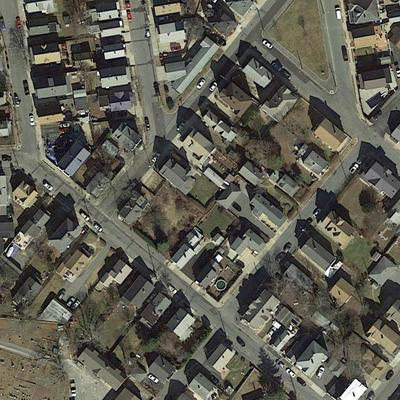
\includegraphics[width=\linewidth]{images/144_1_input_step_513.png}
     \caption{Input Image}
   \end{subfigure}
   %
   \begin{subfigure}[b]{0.3\linewidth}
     
\includegraphics[width=\linewidth]{images/144_2_true_step_513.png}
     \caption{True Label}
   \end{subfigure}
   %
   \begin{subfigure}[b]{0.3\linewidth}
     
\includegraphics[width=\linewidth]{images/144_3_pred_epoch_073_step_38035.png}
     \caption{Prediction}
   \end{subfigure}
   \caption{Example image with prediction obtained from a U-Net trained on ETH-data, \textit{GMaps-public} and \textit{GMaps-custom}.} 
   \label{fig:example}
   \vspace{-6mm}
 \end{figure}

The remainder of this report is structured as follows: In Section \ref{section:data}, we describe the data we used and image augmentations we applied. Section \ref{section:models} presents our baseline models, describes the experiments we conducted to improve on these baselines and extensively elaborates on the contributions of model architecture. Our proposed post-processing techniques are explained and demonstrated in Section \ref{section:post}. Finally, results are compared in Section \ref{section:results} and discussed in Section \ref{section:discussion}.
\section{Data}  \label{section:data}
For this project, ETH provided 100 labelled aerial \acrshort{rgb} images of size 400 by 400 pixel, acquired from Google Maps. Since deep learning approaches often require a large amount of training data, we pursued two strategies to enlarge the data set for training our models.

\subsection{Augmentations}

First, we applied several transformations to each image using the python \textit{Albumentations} library \cite{albumentations}. We applied rotations and flips to make the model more robust against variations in road orientation. In in order to keep the absolute widths of roads, cars, trees etc. fixed, we didn't consider cropping and resizing transformations. These augmentations increased the data set by a factor of eight.

%First, we applied several transformations to each image using the python \textit{Albumentations} library \cite{albumentations}. We applied rotations and flips. In in order to keep the absolute widths of roads, cars, trees etc. fixed, we didn't consider cropping and resizing transformations. These augmentations increased the data set by a factor of eight. An additional benefit is that the model becomes more robust against variations in road orientation.
Additionally, we applied random transformations during training, which are described in Section \ref{section:models}.


\subsection{Additional Data Sets}

Because the provided data set is not only small, but also lacks diversity, we included a publicly available data set which we found on Github \cite{jkfrie}, which was retrieved from Google Maps (2411 images). In the following, we refer to this data set as \textit{GMaps-public}.

We additionally scraped our own images from Google Maps using the tool of \cite{jkfrie} where we focused on including a more diverse set of roads: 1) Roads with a red, light blue, light yellow, white, black and grey color tone, 2) Roads of different quality, e.g. including  some with a lot of cracks, some with unusual texture and some without surface markings. The contribution of these different data sets are evaluated in Section \ref{section:models}. In the following, we refer to this data set as \textit{GMaps-custom}. This set contains 2366 images.

\subsection{Labels}
Even though we have pixel-level labels for our training images, our task is to predict one label per 16x16-pixel patch. We  experimented with approaches to directly predict the label per patch. However, we came to the conclusion that both visually and in terms of prediction accuracy, a pixel-level prediction with subsequent voting per patch with a threshold of 25\% produces better results.  
That is, if at least 25\% of the pixels in a 16x16 px patch are classified as road, the entire patch is classified as a road.
% Describe your idea and how it was implemented to solve the problem. Survey the related work, giving credit where credit is due.
\section{Models and Methods} \label{section:models}

\subsection{Baseline Models}

We have focused on two different model architectures as our baselines: \acrshort{unet} \cite{unet} and \acrshort{gcdcnn} \cite{gcdcnn}.

\subsubsection{Baseline U-Net}
A U-Net is based on a fully connected CNN and consists of a contracting and an expanding path, arranged symmetrically in a U-shape. The contracting path has the architecture of a typical \acrshort{cnn}, it repeatedly applies convolutions and pooling operations to extract meaningful features. This results in reduced spatial information. By combining these features with high-resolution information from the contracting path, the expanding path is able to precisely locate detected objects on a high-resolution output mask. This propagation of context information between different levels in the network is enabled by skip connections.
\subsubsection{Baseline \acrshort{gcdcnn}}
%\subsubsection{\acrshort{gcdcnn}}

The \acrfull{gcdcnn} builds upon the structure of a U-Net. Encoder blocks in the contracting path are replaced by \acrlong{rdb}s (\acrshort{rdb}s) to further enlarge the receptive field, by using the dilation technique \cite{dumoulin2016guide}. A dilated convolution leaves a specific number of pixels spare between the rows and columns of a filter. Residual blocks have been introduced in \cite{residual}, and are used to facilitate information propagation by adding shortcut connections to jump over layers. Additionally, a \acrfull{ppm} is used in the bottleneck layer, which applies multilevel global average pooling to obtain a global representation. See Figure \ref{fig:ppm} in the appendix for an illustration.



In order to improve the two baseline models and to tailor them to our specific problem of segmenting roads on aerial images, we conducted the following experiments. For each experiment, we provide an intuition on why it might improve our model and draw conclusions. This results in our final versions of the \acrshort{unet} and the \acrshort{gcdcnn} compared in Section \ref{section:results}.

\textbf{Experimental setup}:
We train each network for 200 epochs and save the model weights of the best epoch in terms of validation accuracy. We use the optimizer Adam and the dice-loss as our loss function. As initial learning rates, we use $10^{-3}$ for the U-Net and $10^{-4}$ for the \acrshort{gcdcnn}, as we have figured out that these are good values to prevent overfitting as well as divergence. Additionally, we use a learning rate scheduler, which drops the learning rate by a factor of $10$ at epochs $50$ and $100$. We train our models on the ETH data set including the augmented images and on the data set \textit{GMaps-public}. We used a fixed validation set in order to compare validation accuracy among different experiments. Images which contain only non-road pixels are removed from the training set. During training, we apply the transformation \textit{ShiftScaleRotate} with probability 50\% to each image, which is explained in more detail later.

 We evaluate our models in terms of validation accuracy on our validation set and the public score on Kaggle. 

\subsection{Experiment: Training Data}
In this experiment we evaluate the contribution of using additional data described in Section II B. 
% We compare following data sets:
% \begin{itemize}
%     \item \emph{\acrshort{eth} data set}: 800 images (original plus the 8 rotation and flip augmentations) of size (400, 400)
%     \item \emph{GMaps-public}: 2411 images cropped to size (400, 400)
%     \item \emph{GMaps-custom}: X images cropped to size (400, 400)
% \end{itemize}
 We always use a validation set of 20\% and report in Table \ref{tab:datasets} the public score reached on Kaggle as well as the training epoch with the highest validation accuracy. A comparison of the validation accuracy itself is not helpful, since in this experiment the validation set is different for every experiment.
 
\begin{table}[h!]
    \centering
    \begin{tabular}{l|p{0.15\linewidth}|p{0.15\linewidth}}
         Data Set & Public Score & Best Epoch  \\ \hline
         \acrshort{eth} & 89.162 & 77 \\
         GMaps-public & 90.584 & 81 \\
         GMaps-custom & 91.716 & 120 \\ % 20210703-202815-unet_exp_jkfrie_additional
         % GMaps-custom & 91.843 & 173 \\ % 20210708-231725-unet_exp_gmaps_custom
         %\acrshort{eth} + GMaps-public & 91.897 & 142 \\
         %\acrshort{eth} + GMaps-custom & 92.332 & 99 \\
         \acrshort{eth} + GMaps-public + GMaps-custom & \textbf{93.077} & 72 \\ %  20210703-202816-unet_exp_eth_jkfrie_jkfrie_additional
    \end{tabular}
    \caption{Results of training on different data sets (\acrshort{unet})}
    \label{tab:datasets}
    \vspace{-3mm}
\end{table}


The results clearly show that using more data as well as a diverse set of images as in the union of all three sets can lead to a great improvement in prediction accuracy.


\subsection{Experiment: Augmentations During Training}

In order to achieve better generalization and to make our models robust against small variations in the training images, we apply different random augmentations during training. Here we compare the augmentations \acrfull{ssr}, \acrfull{rc} and \acrfull{gn} from the albumentations library \cite{albumentations} using default parameters.


We apply each augmentation with probability 50\% if we use one or two augmentations simultaneously. When using three augmentations, we apply each with probability 40\%. The results are shown in Table \ref{tab:aug}.

\begin{table}[h!]
    \centering
    \begin{tabular}{l|l|p{0.15\linewidth}|p{0.15\linewidth}|p{0.1\linewidth}}
        Model & Method & Validation Accuracy  & Public Score & Best Epoch  \\ \hline
        % results with 2080Ti:
        U-Net & no augmentation & 96.894 & 91.935 & 51 \\ % 20210709-232120-0000_unet_exp_augmentation
        &SSR & 97.185 & 92.352 & 124 \\ % 20210709-163934-0004_unet_exp_augmentation
        % &SSR+CS & 97.189 & 92.138 & 195 \\ % 20210709-163933-0403_unet_exp_augmentation
        &SSR+RC & \textbf{97.202} & \textbf{92.687} & 83 \\ % 20210709-231921-0409_unet_exp_augmentation
        &SSR+RC+GN & 97.145 & 92.510 & 177  \\ % 20210709-163933-040908_unet_exp_augmentation
        % results with 1080Ti:
        %&- & 96.90 & 92.263 & 52 \\ % 20210622-163346-0000_unet_exp_augmentation
        %&SSR & 97.17 & 92.428 & 106 \\ % 20210622-203049-0004_unet_exp_augmentation
        %&SSR+CS & \textbf{97.237} & 92.156 & 107 \\ % 20210624-101058-0403_unet_exp_augmentation
        %&SSR+RC & 97.188 & 92.412 & 83 \\ % 20210625-091625-0409_unet_exp_augmentation
        %&SSR+RC+GN & 97.175 & \textbf{92.549} & 177 \\ % 20210625-053145-040908_unet_exp_augmentation
        \hline
        GC-DCNN & no augmentation & 97.004 & 91.256 & 56 \\ % 20210626-123903-0000_gcdcnn_exp_augmentation
        & SSR & 97.270 & 92.242 & 71 \\ % 20210626-222336-0004_gcdcnn_exp_augmentation
        & SSR+RC & \textbf{97.309} & 92.317 & 155 \\ % 20210627-171426-0409_gcdcnn_exp_augmentation
        & SSR+RC+GN & 97.273 & \textbf{92.422} & 95 \\ % 20210627-171254-040908_gcdcnn_exp_augmentation
    \end{tabular}
    \caption{Results of Augmentation Experiments for U-Net and GC-DCNN}
    \label{tab:aug}
        \vspace{-5mm}
\end{table}
\subsection{Experiment: Architecture Alterations U-Net}
\label{section:unetplus}
In order to fine tune the U-Net architecture to our specific task, we experimented with varying dilation,  convolutional filter sizes and max pooling kernel sizes. 
%As shown in Table \ref{tab:unet_alt} in Appendix  such model changes did not contribute much to prediction accuracy in our case.
Table \ref{tab:unet_alt} in the Appendix shows the variations and results in detail. The best architecture, henceforth referred to as \acrshort{unet}-Plus, was obtained using a pooling kernel of size 4 which increased the public score (in \%) by 0.457. 
 
%In order to adapt the basic U-Net architecture to our specific task, we applied several changes in architecture and hyper parameters. We experimented with increasing dilation, varying convolutional filter sizes and max pooling kernel sizes. 


\subsection{Experiment: Architecture Alterations \acrshort{gcdcnn}}\label{section:gcdcnnplus}

We experimented with the following alterations to the \acrshort{gcdcnn} architecture. 
\paragraph{Deep} The original \acrshort{gcdcnn} was designed for images of size 256x256. However, as we use images of size 400x400, the bottleneck layer has a higher resolution. Therefore, we study the effect of a deeper network. Instead of 3 \acrshort{rdb}s with filters [128, 256, 512] we use 4 \acrshort{rdb}s with an additional filter of size 1024. This reduces the image size in the bottleneck layer by a factor of 16.
\paragraph{\acrfull{aspp}} We replace the bridge (\acrshort{ppm}) with the \acrshort{aspp} \cite{aspp_7913730} module.
\paragraph{Attention} We use an attention gate, as proposed by Oktay et al. \cite{oktay2018attention}, in the expanding path of the \acrshort{gcdcnn}. For this, we apply the attention gate to the decoder tensors before concatenating them with the skip connections.

%Finally we combine these alterations to find the best combination. The results, that can be found in the Appendix in Table \ref{tab:gcdcnn_tuning}, show that the improvements are only of small degree. 

%We combine these alterations to find the best novel combination:
%\acrshort{gcdcnn}-plus. The results in Table \ref{tab:gcdcnn_tuning} in the Appendix show an improvement of 0.049 in Validation Accuracy and 0.307 in Public Score. 

The best result is obtained by combining all three above-mentioned alterations which creates our novel altered model \acrshort{gcdcnn}-plus. The results in Table \ref{tab:gcdcnn_tuning} in the Appendix show that our architecture variations can increase the public score by up to 0.307 percentage points.


\section{Post-processing} \label{section:post}
We observed recurring visual artefacts like disconnected road fragments, see Fig. \ref{fig:example} c), in our predicted results. Initially we attempted to resolve this using classical methods such as morphological operations (e.g. erosion, dilation) and median filtering. While these structure based approaches helped by connecting disjoint road segments, they introduced new artefacts in some predictions by merging adjacent roads. Due to the diversity of the images, the exact filter type, shape and size, which worked best for a prediction was sensitive to the road structure. Instead of a manual grid search for the best possible parameters per image, we developed two novel learning based post processing methods.

\begin{figure}
\centering
%   \begin{subfigure}[b]{0.3\linewidth}
%     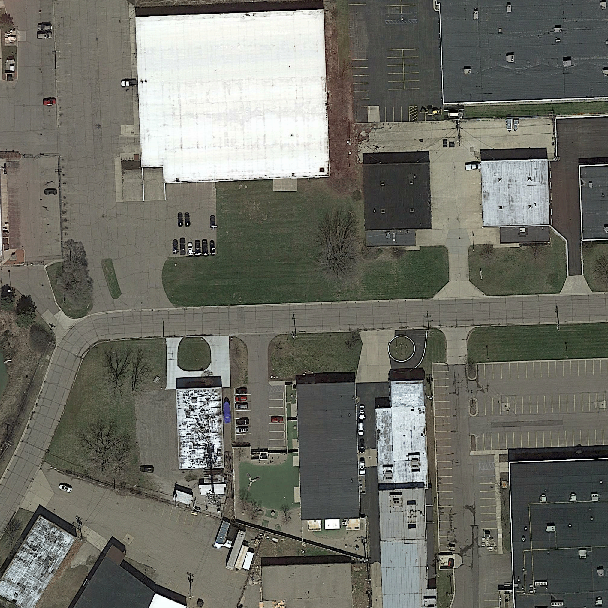
\includegraphics[width=\linewidth]{images/test_105.png}\caption{}
%   \end{subfigure}
  %
  \begin{subfigure}[b]{0.3\linewidth}
    
\includegraphics[width=\linewidth]{images/pred_190_orig.png}
    \caption{}
  \end{subfigure}
  %
  \begin{subfigure}[b]{0.3\linewidth}
    
\includegraphics[width=\linewidth]{images/pred_190_simpleunet.jpg}
    \caption{}
  \end{subfigure}
     \begin{subfigure}[b]{0.3\linewidth}
     
\includegraphics[width=\linewidth]{images/pred_190_pconv_dil3.jpg}
     \caption{}
   \end{subfigure}
  
%   \par\smallskip
%   \begin{subfigure}[b]{0.3\linewidth}
%      
\includegraphics[width=\linewidth]{images/dil_5_pred_105.jpg}\caption{}
%   \end{subfigure}

%   \begin{subfigure}[b]{0.3\linewidth}
%      
\includegraphics[width=\linewidth]{images/dil_7_pred_105.jpg}\caption{}
%   \end{subfigure}
  \caption{Retrain on binary predictions: 
  a) Original prediction, b) Retrain simple \acrshort{unet},
  c) Retrain \acrshort{unet} with partial convolution and dilation 3.
  }
  \label{fig:postprocessing}
  \vspace{-7mm}
\end{figure}


\subsection{Retraining on binary predicted images} \label{subsec:binary_retraining}
We used the best predictions of the U-Net \& \acrshort{gcdcnn} as a training set and retrained the network to learn how to connect roads by joining lines and to remove noisy predictions.

\subsubsection{Partial convolution} 
Partial convolution layers are commonly used for image inpainting of irregular holes \cite{partialconv}. Instead of learning different morphological filters, we decided to use these layers to inpaint pixels to recreate road images.
%Partial convolutions normalize the output to adjust for a fraction of the missing data. 
When retraining on the binary images, we replaced the normal convolution layers with partial convolution layers as in \cite{partialconv}. 
As seen in Figure \ref{fig:postprocessing} c) this leads to cleaner boundaries between roads and denoised predictions.

\subsubsection{Increasing the receptive field} As seen in Fig. \ref{fig:postprocessing} b), some of the roads still remained disconnected. Increasing the dilation helped to increase the receptive field of the network to learn whether disjoint segments separated by a large black margin indeed constitute a road. This improved the quality of predicted images both for the \acrshort{unet} with partial convolution and the normal \acrshort{unet} as shown in Tables \ref{tab:postprocessingunet} and \ref{tab:postprocessinggcdcnn} in the Appendix. Retraining helped to produce cleaner images, but improved the public score by only 0.199 percentage points due to the 16x16 patch abstraction.

\subsection{Learning with Hough Transformations}
 Another idea we came up with was to nudge the network towards predicting connected roads by explicitly presenting possible connected line fragments. A classical computer vision technique to detect shapes such as lines in images is the so-called Hough transformation \cite{hough}. By looking at the predicted mask and counting the number of pixels that lie on straight lines in specific angles, this method returns all possible lines that exceed a certain threshold. We draw these lines with the width of an average street on the predicted masks, concatenate this image with the prediction and the original RGB image and train a post-processing network (U-Net) on it. Thus, our model is trained on images with 5 channels (RGB, prediction, lines). The network should decide which of these roads (if any) it should keep. 

 This can be interpreted in several different ways. First, one could see it as letting the network learn how to remove predicted roads, thereby concentrating exactly on the parts between already identified road fragments. Secondly, one could also interpret this as a kind of topological prior. The prior probability of another road pixel on the connecting line between two fragments is higher than in any other part of the image. Thirdly, by providing these lines, we give the network an additional set of features, which can be used to improve the current predictions – or can be ignored.

\begin{figure}[h!]
\centering
  \begin{subfigure}[b]{0.22\linewidth}
    
\includegraphics[width=\linewidth]{images/satImage_024_prediction.png}\caption{}
  \end{subfigure}
  %
  \begin{subfigure}[b]{0.22\linewidth}
    
\includegraphics[width=\linewidth]{images/satImage_024_lines.png}\caption{}
  \end{subfigure}
%
   \begin{subfigure}[b]{0.22\linewidth}
    
\includegraphics[width=\linewidth]{images/satImage_075.png}\caption{}
  \end{subfigure}
  %
  \begin{subfigure}[b]{0.22\linewidth}
    
\includegraphics[width=\linewidth]{images/satImage_075-lines.png}\caption{}
  \end{subfigure}
    \caption{Hough Transformations: (a), (c) show the original predictions. (b), (d) show the completed lines.
  %A U-Net is trained on these three images (5-channels) to decide whether to keep the completed lines.
  }
  \label{fig:hough}
\end{figure}

For an illustration of the Hough Transformation, see Fig. \ref{fig:hough}. In the first image (a, b), we see that the lines are very simple and therefore this approach works fine. However, when the road network is more complicated as in (c), there are many wrong lines (d). This leads our model to use the original prediction and mostly ignore the lines. Therefore, this post-processing technique does not help in improving prediction accuracy.

% Further work could be done by including the Hough Transformation lines in the training of the main network in form of a prior, starting in a certain epoch.

\subsection{Ensemble Methods}

Averaging the predictions from different models is another form of post-processing, as it helps to remove artefacts, such as separated road predictions. If at least 50\% of the models predicted a pixel as road, then the ensemble prediction considers it to be road. Afterwards, the predictions are patched as usual. This procedure has shown to significantly improve prediction accuracy, as shown in Section \ref{section:results}.

%   Show evidence to support your claims made in the introduction.

\section{Results} \label{section:results}

Table \ref{tab:results} summarizes the results of our final models by comparing the Public Scores on Kaggle.
The trend is that our proposed post-processing technique  (Retrain on binary, \ref{subsec:binary_retraining}) improves the accuracy. The best results are obtained with an ensemble of the best predictions from each model specification. For the ensemble, post-processing did not improve the accuracy. A reason might be the already removed artefacts by the ensemble.

%However using post-processing on the ensemble results reduces the accuracy. Our intiution is that the possible corrections in artefacts could have already been taken care of by the ensemble.

%Postprocessing with the retrained partial convolution network (\ref{subsec:binary_retraining}) improved the accuracy, but not for the ensemble prediction. A reason might be the already removed artefacts by the ensemble.  

\begin{comment}
\begin{table}[h!]
    \centering
    \begin{tabular}{p{0.4\linewidth}|p{0.3\linewidth}|p{0.2\linewidth}}
    \hline
    \hline
         Model & Data Sets & Public Score \\
         \hline
         U-Net Baseline & ETH + GMaps-public  & 92.352\\
         \hline
         \parbox[t]{\linewidth}{U-Net + Augment.: SSR + RC}  & \parbox[t]{\linewidth}{ETH, GMaps-public,\\ GMaps-custom}  & 92.689 \\ % 20210710-115821-unet_final
         \hline
         \parbox[t]{\linewidth}{U-Net-Plus + Augment.: SSR + RC} & \parbox[t]{\linewidth}{ETH, GMaps-public,\\ GMaps-custom} & 92.835 \\ % 20210710-115820-unet_final_plus
         \parbox[t]{\linewidth}{+ postprocessing } &  & 93.034 \textcolor{green}{*}\\
         \hline
         GC-DCNN Baseline & ETH + GMaps-public  & 92.242 \\
         \hline
         \parbox[t]{\linewidth}{GC-DCNN\\ + Augment.: SSR + RC + GN} & \parbox[t]{\linewidth}{ETH, GMaps-public,\\ GMaps-custom}  & 92.457 \\ % 20210710-115819-gcdcnn_final
         \hline
         \parbox[t]{\linewidth}{GC-DCNN-Plus\\ + Augment.: SSR + RC + GN} & \parbox[t]{\linewidth}{ETH, GMaps-public,\\ GMaps-custom}  & 92.999 \\
         \parbox[t]{\linewidth}{+ postprocessing} &  & 93.065  \textcolor{green}{*}\\

    \hline
    %\hdashline
    % \hline
    % U-Net Ensemble (5 different lr-schedules) & ETH + GMaps-public  & \textcolor{red}{\textbf{93.198}} \\ 
    \parbox[t]{\linewidth}{Ensemble: \\GC-DCNN Baseline, U-Net Baseline, GC-DCNN,\\ U-Net, GC-DCNN plus, \\ U-Net plus } & & \textbf{93.497} \\
    \parbox[t]{\linewidth}{+ postprocessing} &  & 93.303\\
    \hline
    \hline
    \end{tabular}
    \centering
    %\caption{Results of Final Models: The \acrshort{unet}-plus refers to using PoolKernel (4) and the \acrshort{gcdcnn}-plus to the alternations: ASPP + Attention + Deep. Postprocessing refers to using the retrained partial convolution network (see \ref{subsec:binary_retraining}) on the predicted masks.}
    \caption{Results of Final Models: \acrshort{unet}-plus Sec: \ref{section:unetplus}, \acrshort{gcdcnn}-plus Sec: \ref{section:gcdcnnplus}, \textcolor{green}{*} Postprocessing Sec:  \ref{subsec:binary_retraining})}
    \label{tab:results}
        \vspace{-4mm}
\end{table}
\end{comment}

\begin{table}[h!]
    \centering
    \begin{tabular}{p{0.22\linewidth}|p{0.31\linewidth}|p{0.14\linewidth}|p{0.03\linewidth}|p{0.08\linewidth}}
    \hline
    \hline
         Model & Specification & Data Sets  & PP & Public Score \\
         \hline
         U-Net &  Baseline  & \circ{1}, \circ{2} & -  & 92.352\\
         \hline
         U-Net & Aug.: SSR + RC & \circ{1}, \circ{2}, \circ{3} & - & 92.689 \\ % 20210710-115821-unet_final
         \hline
         U-Net-plus & Aug.: SSR + RC  & \circ{1}, \circ{2}, \circ{3} & - & 92.835 \\ % 20210710-115820-unet_final_plus
          &  & & \checkmark & 93.034 \\
         \hline
         GC-DCNN  & Baseline  & \circ{1}, \circ{2} & - & 92.242 \\
         \hline
         GC-DCNN & Aug.: SSR + RC + GN & \circ{1}, \circ{2}, \circ{3} & - & 92.457 \\ % 20210710-115819-gcdcnn_final
         \hline
         GC-DCNN-plus & Aug.: SSR + RC + GN & \circ{1}, \circ{2}, \circ{3} & - & 92.999 \\
         & & & \checkmark   & 93.065\\

    \hline
    % \parbox[t]{\linewidth}{GC-DCNN Baseline, \\ U-Net Baseline, \\ GC-DCNN,\\ U-Net, \\ GC-DCNN plus, \\ U-Net plus }
    Ensemble &  All models from above, not post-processed &  & - & \textbf{93.497} \\
     & &  & \checkmark  & 93.303\\
    \hline
    \hline
    \end{tabular}
    \centering
    %\caption{Results of Final Models: The \acrshort{unet}-plus refers to using PoolKernel (4) and the \acrshort{gcdcnn}-plus to the alternations: ASPP + Attention + Deep. Postprocessing refers to using the retrained partial convolution network (see \ref{subsec:binary_retraining}) on the predicted masks.}
    \caption{Results of Final Models: \acrshort{unet}-plus Sec: \ref{section:unetplus}, \acrshort{gcdcnn}-plus Sec: \ref{section:gcdcnnplus}, PP: Post-processing Sec:  \ref{subsec:binary_retraining}). Data sets: \circ{1} ETH, \circ{2} GMaps-public, \circ{3} GMaps-custom.}
    \label{tab:results}
\end{table}

  \vspace{-4mm}
\begin{comment}

\begin{table}[h!]
    \centering
    \begin{tabular}{l|p{0.1\linewidth}|p{0.1\linewidth}|p{0.1\linewidth}|p{0.1\linewidth}|p{0.1\linewidth}|l}
    
    \hline
    \hline
    1 & Model & ETH & GMaps-public & GMaps-custom & Post-Process. & Score
    
    \end{tabular}
    \caption{Results of final models. \textbf{Post} = Post-processing (Retrain on binary images). \textbf{Score} = Public Score on Kaggle}
\end{table}


\end{comment}

% Discuss the strengths and weaknesses of your approach, based on the results. Point out the implications of your novel idea on the application concerned.

\section{Discussion} \label{section:discussion}

We observe that an accurately tuned U-Net performs similar to the more complex \acrshort{gcdcnn} and other variants with slight architecture alterations, suggesting that the exact model architecture plays a minor role. The largest contribution to prediction accuracy was reached by using additional diverse training images. Averaging multiple predictions in an ensemble significantly improves the predictions by removing artefacts and by combining the strengths of several models. Despite not improving Kaggle score significantly, our proposed post-processing method: retraining on binary images with a large receptive field was able to fill small gaps between roads. Since we are evaluated on the patch-level accuracy, these slight improvements did not reflect in the patched predictions. A general drawback of post-processing techniques is their required extra work to train another network.

%We observed that an accurately tuned U-Net performs similarly good, even better than the more complex GC-DCNN and other variants with slight architecture alternations. The observed differences in accuracy are very small, suggesting that the exact model architecture plays only a minor role. The largest contribution to prediction accuracy was reached by using additional training images which are as diverse as possible. Averaging multiple predictions in an ensemble significantly improves the predictions by removing artefacts and by combining the strengths of several models.

%Even though not all of our proposed post-processing techniques were able to improve prediction accuracy, retraining on binary images with a large receptive field was able to fill small gaps between roads and therefore enhance the visual quality of the predictions. Since we are evaluated on the patch-level accuracy, these slight improvements did not reflect on the patch predictions. A general drawback of post-processing techniques is their required extra work to train another network.
% Summarize your contributions in light of the new results.

\section{Summary}

In this project we investigated the contribution of complex model architectures in comparison to other factors and conclude that the exact model architecture plays only a minor role.
Furthermore, we proposed and evaluated two post-processing techniques, which improved our Kaggle public score only slightly, but enhanced the visual quality of the predictions significantly.

%In this project we have investigated the contribution of complex model architectures in comparison to other factors and concluded that the exact model architecture plays only a minor role even when  fine tuned. Furthermore, we proposed and evaluated several post-processing techniques, which were only partly able to improve our Kaggle Public Score, but some methods enhanced the predictions visually by removing artefacts or by connecting road fragments.
\newpage
\appendix

\subsection{\acrlong{ppm}}

\begin{figure}[H]
\centering
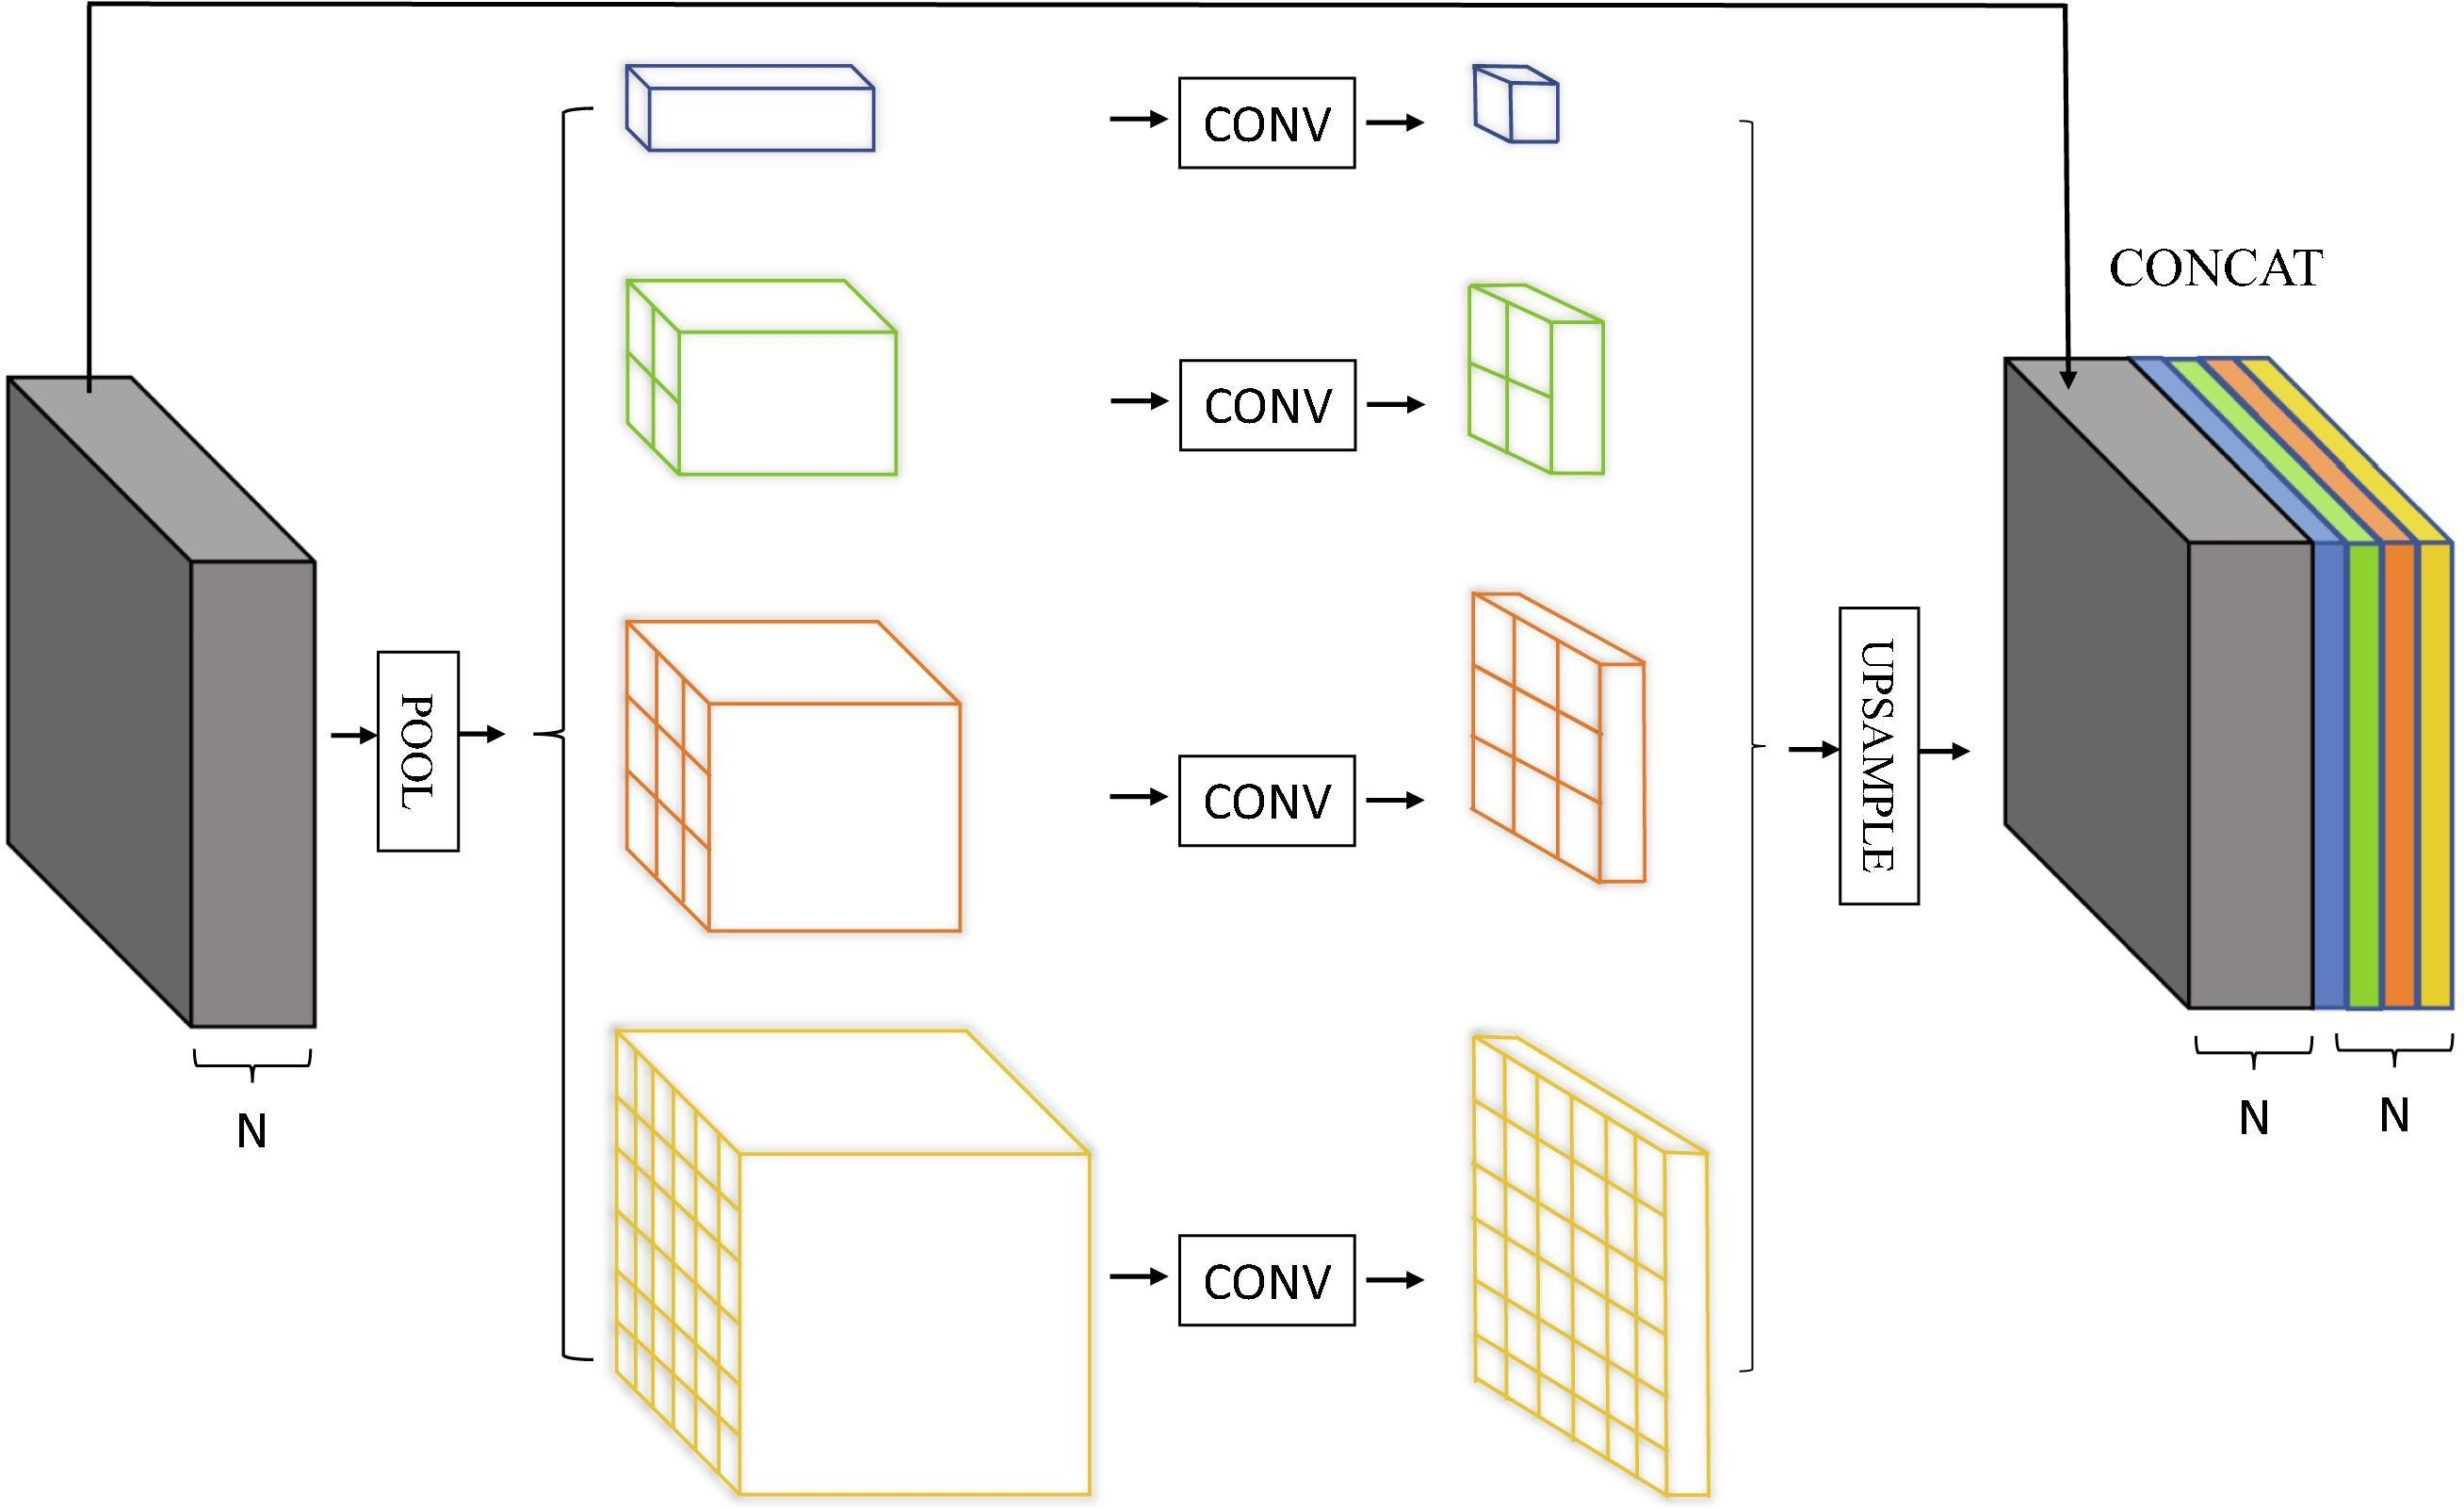
\includegraphics[width=1.0\linewidth]{images/pyrmid-pooling.jpg}
\caption{\acrlong{ppm} used in \acrshort{gcdcnn} \cite{gcdcnn}}
\label{fig:ppm}
\end{figure}

\subsection{Augmentation parameters}
In total we experimented with over twenty different augmentations. A key result of these experiments is, that if \acrfull{ssr} is not applied the model overfits and achieves a training accuracy of over 99\%. For brevity, we here only list the explanation of the top three augmentations.
\begin{itemize}
    \item \acrfull{ssr}: Randomly shift, scale and rotate the image. We uniformly draw a shift value in [-0.0625, 0.0625], a scale value in [-0.1, 0.1] and a rotation value in [-45, 45] degrees. % We use BORDER_REFLECT_101 which mirrors the border...
    % \item \acrfull{cs}: The three channels RGB are shuffled randomly.
    \item \acrfull{rc}: Change the contrast with a random factor in the range  [-0.2, 0.2]
    \item \acrfull{gn}: We apply Gaussian noise with a mean of 0 and a variance limit of [10.0, 50.0]. % not clear what the variance parameter of the Gaussian is set to; maybe a uniformly drawn value from the limit interval?
\end{itemize}

\subsection{Results of architecture alterations}

\subsubsection{U-Net}

In the following we list the explanations of the different \acrshort{unet} architecture tunings of which the results can be found in table \ref{tab:unet_alt}.
\begin{itemize}
    \item Dilation: Dilations with factors 3 and 18 were applied to all filters
    \item Filtersize: Filtersize was increased to 5 instead of 3
    \item PoolKernel: The Max Pooling kernel was increased to size 4 instead of 2
    \item Dilation and LR-Change: Dilation with factor 3 with a initial learning rate of $10^{-4}$ instead of $10^{-3}$
\end{itemize}

\begin{table}[h!]
    \centering
    \begin{tabular}{l|p{0.15\linewidth}|p{0.15\linewidth}|p{0.15\linewidth}}
         method & Validation Accuracy  & Public Score & Best Epoch  \\
         \hline
         Baseline U-Net & \textbf{97.185} & 92.352 & 124\\
         Dilation (3) & 96.817 & 91.942 & 34\\
         Dilation (18) & 96.280 & 90.941 & 86\\
         Filtersize (5) & 97.123 & 92.793 & 105\\
         PoolKernel (4) & 97.169 & \textbf{92.809} & 149\\
         Dilation (3) lr=$10^{-4}$ & 97.110 & 92.203 & 70\\
    \end{tabular}
    \caption{Results of U-Net Architecture Alterations}
    \label{tab:unet_alt}
\end{table}

\subsubsection{GC-DCNN}

%The results in table \ref{tab:gcdcnn_tuning} show that different architecture modifications do not change the validation accuracy by a lot. Considering that the experiments dataset consists of multiple datasets (ETH, GMaps-public) with different ground truth labeling technique, we reason that the validation score is close to the optimal.
Results of architecture variations of the \acrshort{gcdcnn} can be seen in Table \ref{tab:gcdcnn_tuning}. As our final model we choose the model ASPP + Attention + Deep, since it achieved the best validation score as well as a high public score.

\begin{table}[h!]
    \centering
    \begin{tabular}{l|p{0.15\linewidth}|p{0.15\linewidth}|p{0.15\linewidth}}
         Method & Validation Accuracy & Public Score & Best Epoch  \\ \hline
         - & 97.270 & 92.242 & 71 \\ % 20210626-222336-0004_gcdcnn_exp_augmentation
         Attention & 97.279 & 92.246 & 60 \\ % 20210626-093027-gcdcnn_exp_attention
         ASPP & 97.3 & \textbf{92.549} & 97 \\ % 20210626-093027-gcdcnn_exp_aspp_avg_pool
         ASPP + Attention & 97.145 & 92.201 & 51 \\ % 20210626-111758-gcdcnn_exp_aspp_avg_pool_attention
         Deep & 97.272 & 92.195 & 178 \\ % 20210626-092358-gcdcnn_exp_deep
         ASPP + Deep & 97.301 & \textbf{92.468} & 105 \\ % 20210625-200334-gcdcnn_exp_deep_aspp_avg_pool
         Attention + Deep & 97.235  & 92.049 & 102  \\ % 20210625-215203-gcdcnn_exp_deep_attention
         ASPP + Attention + Deep & \textbf{97.319} & \textbf{92.430} & 132 \\ % 20210625-205535-gcdcnn_exp_deep_aspp_avg_pool_attention
    \end{tabular}
    \caption{Results of \acrshort{gcdcnn} Architecture Alterations}
    \label{tab:gcdcnn_tuning}
\end{table}


%  \begin{table}[h!]
%      \centering
%      \begin{tabular}{l|l|p{0.10\linewidth}|p{0.10\linewidth}|p{0.05\linewidth}}
%           Model & Validation Acc & Public Score & Dilation\\ \hline
%     UNET &  0.97563 & - & -\\\hline % 20210704-202654-unet_exp_template
%     Retrain UNET &  0.98141 & - & 1\\ % 20210706-174459-unet_exp_template
%     Retrain UNET  & 0.98146  & - & 5\\ % 20210706-175301-unet_exp_dilation_5
%     Retrain UNET &  0.98148 & - & 7\\ %20210706-175332-unet_exp_dilation_7
%     \hline
%     Retrain UNET-PCONV & 0.98165 & - & 1\\ %20210707-213909-unet_pconv_exp_template
%     Retrain UNET-PCONV & 0.98142 & - & 3\\ %20210707-215537-unet_pconv_exp_dilation_3
%     Retrain UNET-PCONV & 0.98149 & - & 5\\ %20210707-215538-unet_pconv_exp_dilation_5
%     Retrain UNET-PCONV & 0.98148 & - & 7\\ %20210707-215539-unet_pconv_exp_dilation_7
%      \end{tabular}
%      \caption{Results of retraining on binary images}
%      \label{tab:postprocessing}
%  \end{table}
 
\subsection{Postprocessing results}
 
\begin{table}[H]
    \centering
    \begin{tabular}{l|p{0.15\linewidth}|p{0.15\linewidth}|p{0.10\linewidth}}
        Model & Validation Accuracy & Public Score & Dilation\\ \hline
        \acrshort{unet}-plus &  96.150 & 92.835 & -\\\hline % 
        Retrain \acrshort{unet} & \textbf{97.433} & 92.964 & 1\\ % 
        Retrain \acrshort{unet}  &  97.449 & \textbf{93.034} & 5\\ % 
%        Retrain \acrshort{unet} &  97.410 & 92.961 & 7\\ %
        \hline
        Retrain \acrshort{unet}-PCONV & 97.439 & 92.987 & 1\\ %
        Retrain \acrshort{unet}-PCONV & 97.450 & 93.001 & 3\\ %
        Retrain \acrshort{unet}-PCONV & 97.422 & 93.028 & 5\\ %
%        Retrain \acrshort{unet}-PCONV & 97.429 & 92.999 & 7\\ %
    \end{tabular}
    \caption{Results of postprocessing binary retraining using \acrshort{unet} on \acrshort{unet}-plus predictions}
    \label{tab:postprocessingunet}
\end{table}
 
 
\begin{table}[H]
    \centering
    \begin{tabular}{l|p{0.15\linewidth}|p{0.15\linewidth}|p{0.10\linewidth}}
        Model & Validation Accuracy & Public Score & Dilation\\ \hline
        GCDCNN-plus&  96.28 & 92.99 & -\\\hline % 
        Retrain \acrshort{unet} &  97.484 & 93.032 & 1\\ % 
        Retrain \acrshort{unet}  & 97.480  & \textbf{93.065} & 5\\ % 
%        Retrain \acrshort{unet} &  97.493 & 93.041 & 7\\ %
        \hline
        Retrain \acrshort{unet}-PCONV & 97.490 & 93.041 & 1\\ %
        Retrain \acrshort{unet}-PCONV &  97.547 & 93.038 & 3\\ %
        Retrain \acrshort{unet}-PCONV & \textbf{97.485} & 93.029 & 5\\ %
%        Retrain \acrshort{unet}-PCONV &  97.493 & 93.029 & 7\\ %
    \end{tabular}
    \caption{Results of postprocessing binary retraining using \acrshort{unet} on \acrshort{gcdcnn}-plus predictions}
    \label{tab:postprocessinggcdcnn}
\end{table}







\bibliographystyle{IEEEtran}
\bibliography{DeepLearners-literature}

\glossarystyle{altlist}
\printglossary[type=\acronymtype]

\end{document}
